\documentclass[UTF8,11pt,a4paper]{ctexart}

\usepackage[a4paper,top=2.3cm,bottom=2.2cm,left=2.45cm,right=2.45cm,headheight=15pt]{geometry}
\usepackage{amsmath,amssymb}
\usepackage{array,booktabs,longtable,tabularx}
\usepackage{graphicx}
\usepackage{float}
\usepackage{xcolor}
\usepackage{hyperref}
\usepackage{url}

\definecolor{AegisBlue}{HTML}{1F4E79}
\definecolor{AegisTeal}{HTML}{147D92}
\hypersetup{
  colorlinks=true,
  linkcolor=AegisBlue,
  citecolor=AegisTeal,
  urlcolor=AegisBlue,
  pdfauthor={AegisKV Project Team},
  pdftitle={AegisKV Agent-Aware LLM Inference Fault-Tolerance System Design},
  pdfsubject={Project acceptance design document}
}

\setlength{\parindent}{2em}
\setlength{\parskip}{0.15em}
\setlength{\emergencystretch}{3em}
\renewcommand{\arraystretch}{1.22}
\setcounter{tocdepth}{2}
\pagestyle{headings}

\newcommand{\systemname}{\textsc{AegisKV}}

\begin{document}

\hypersetup{pageanchor=false}
\begin{titlepage}
  \centering
  \vspace*{1.7cm}
  {\color{AegisBlue}\rule{\textwidth}{1.1pt}}\\[0.9cm]
  {\zihao{1}\bfseries AegisKV 项目验收设计文档\par}
  \vspace{0.5cm}
  {\zihao{3}\bfseries 面向 Agentic LLM Workflow 的大模型推理容错系统\par}
  \vspace{0.9cm}
  {\color{AegisBlue}\rule{\textwidth}{1.1pt}}\\[1.4cm]

  \begin{tabular}{>{\bfseries}p{3.5cm}p{8.6cm}}
    文档状态 & 当前正式设计基线 \\
    设计范围 & 底层 GPU failure、整请求跨 DP 重试、DP$\times$PP 部署 \\
    编制单位 & AegisKV 项目组 \\
    编制日期 & 2026 年 8 月 6 日 \\
    分发范围 & 合作双方授权的技术、验收与知识产权人员 \\
  \end{tabular}
  \vfill
\end{titlepage}

\hypersetup{pageanchor=true}
\pagenumbering{Roman}

\section*{摘要}
\addcontentsline{toc}{section}{摘要}

Agentic 应用将多轮推理、工具调用和并行智能体组织为工作流。长上下文使 GPU 故障后的
前缀重算越来越昂贵，而工作流依赖又使相同的请求恢复时间产生不同的 workflow
completion time（WCT）影响。\systemname{} 以工作流级故障影响为出发点，通过三个
相互衔接的算法实现选择性 KVCache 保护：Algorithm 1 根据工作流执行图计算请求
Slack；Algorithm 2 在 KV chunk 到达时比较恢复收益与备份成本，选择 GPU、Host 或
Recompute；Algorithm 3 根据上一控制窗口的需求、实际占用和未满足收益，调整每个
DP 的 HBM 比例 $\alpha$ 与 Host DRAM 比例 $\beta$。系统只在正常路径开销可接受时
实施保护，并在 GPU failure 后把受影响请求迁移到健康 DP，复用已备份 KV 或重算
未覆盖部分。

\textbf{关键词：}Agentic Serving；工作流感知；GPU 故障恢复；KVCache；WCT

\clearpage
\tableofcontents
\clearpage
\pagenumbering{arabic}

\section{背景、问题与目标}

\subsection{问题背景}

Agentic 请求通常重复经历 prompt、thinking、tool call、tool result 和下一轮推理。
工具返回后，应用以新增内容和历史会话作为新的推理输入，因此前缀随工作流推进持续
增长。若执行 GPU 在较晚阶段失效且 KVCache 只存在于该 GPU，请求需要在健康 GPU 上
重新排队并重新计算较长前缀。与此同时，工作流可能包含串行主链和并行 subagent；
某个请求是否拖慢最终 WCT，取决于它所处的依赖关系，而不仅取决于 KV 大小。

现有系统已分别研究分页 KV、前缀复用、分层缓存和 agentic workflow 调度
\cite{kwon2023vllm,zheng2024sglang,qin2025mooncake,lin2024parrot,
pan2025kvflow,luo2026agentix,yu2026pythia}，也有工作研究 KV 流式复制和 LLM 恢复
\cite{strati2024dejavu,jayakody2026ghostserve,cao2026lumen}。本文关注的联合问题是：
如何把应用层工作流依赖转化为请求 Slack，并在有限 HBM、Host DRAM 与正常服务预算
下，持续选择最值得保护的 KV chunk。

\subsection{动机观察}

Real CC trace\cite{semianalysis2026cctraces} 中，并行 subagent 的执行时间存在明显差异。
在 393 个 workflow 的 321 次并行 fan-out 中，最慢/最快分支时长比的中位数为
$2.2\times$，P90 为 $8.6\times$。fan-in 必须等待最慢分支，因此保护资源应优先
用于故障延迟会传播到当前最长路径的请求。

\begin{figure}[H]
  \centering
  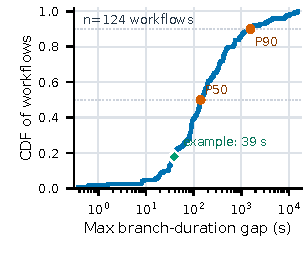
\includegraphics[width=\textwidth]{../figures/real-cc-parallel-subagent-duration.pdf}
  \caption{Real CC trace 中并行 subagent 的执行时长分布。}
  \label{fig:real-cc-parallel}
\end{figure}

受控模拟还显示：上下文越长，从头重算的恢复代价越大；即使丢失相同规模的 KV，
故障发生在不同工作流位置时，对 WCT 的影响也不同。两组实验只用于说明设计动机，
不作为完整系统的最终性能结论。

\begin{figure}[H]
  \centering
  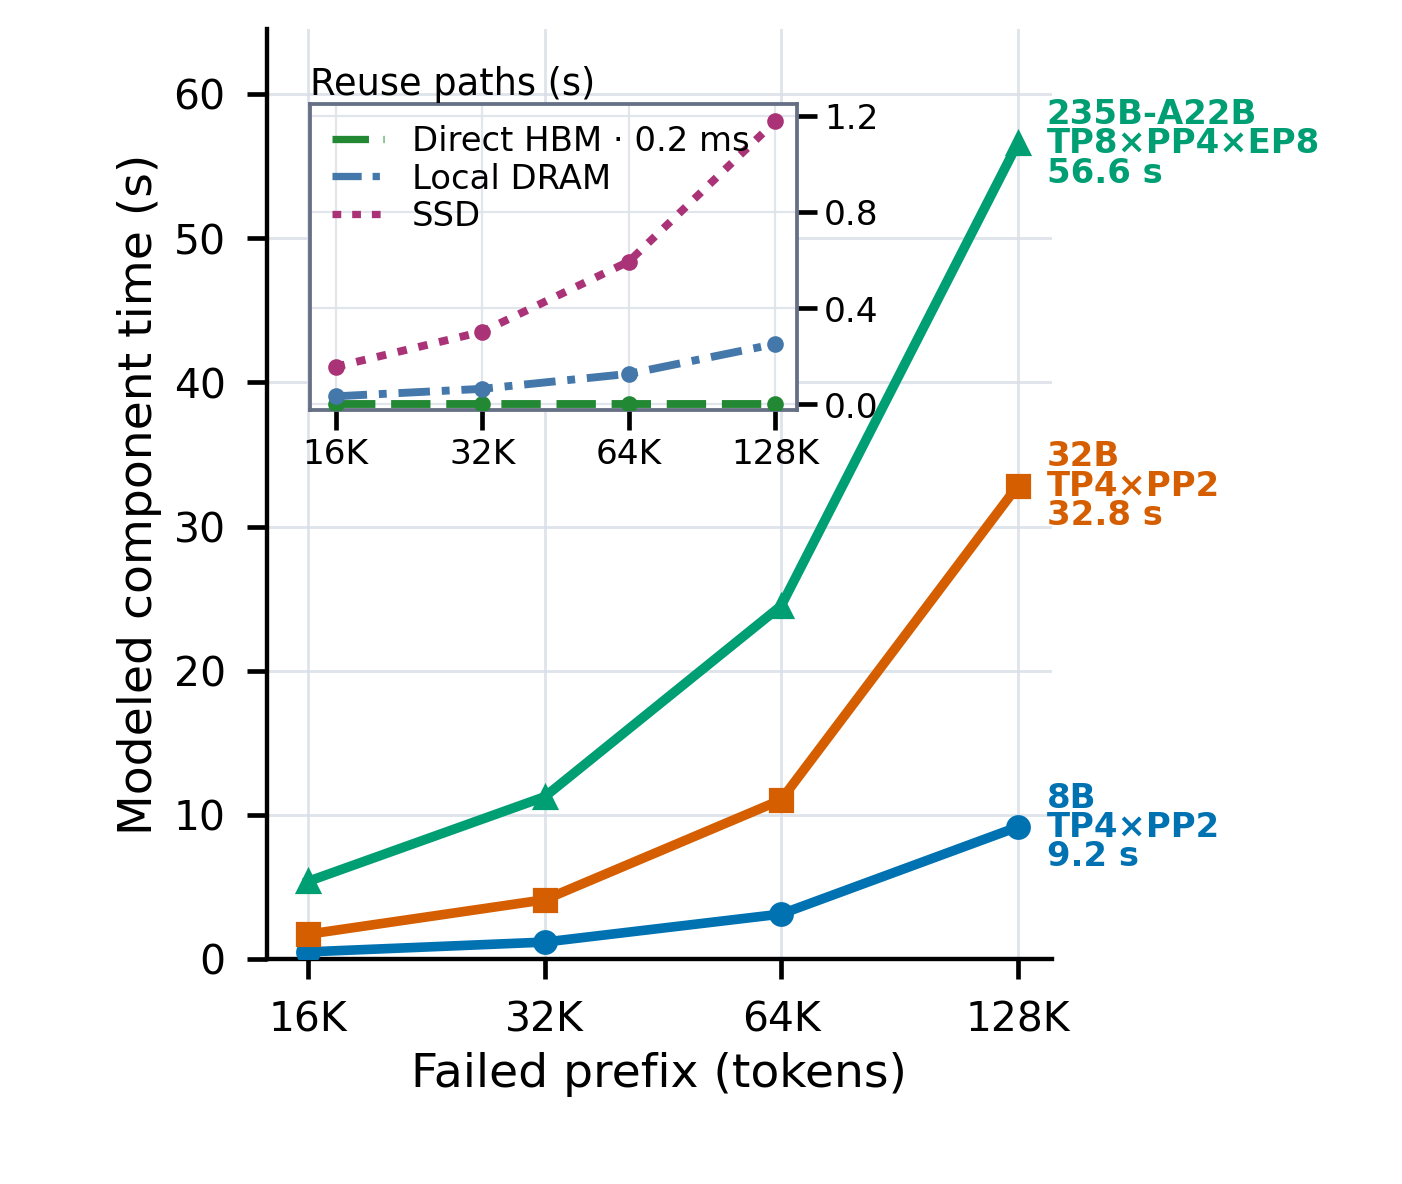
\includegraphics[width=0.96\textwidth]{../figures/motivation-recovery-scaling.png}
  \caption{上下文规模与故障恢复时间的受控模拟。}
  \label{fig:motivation-recovery-scaling}
\end{figure}

\begin{figure}[H]
  \centering
  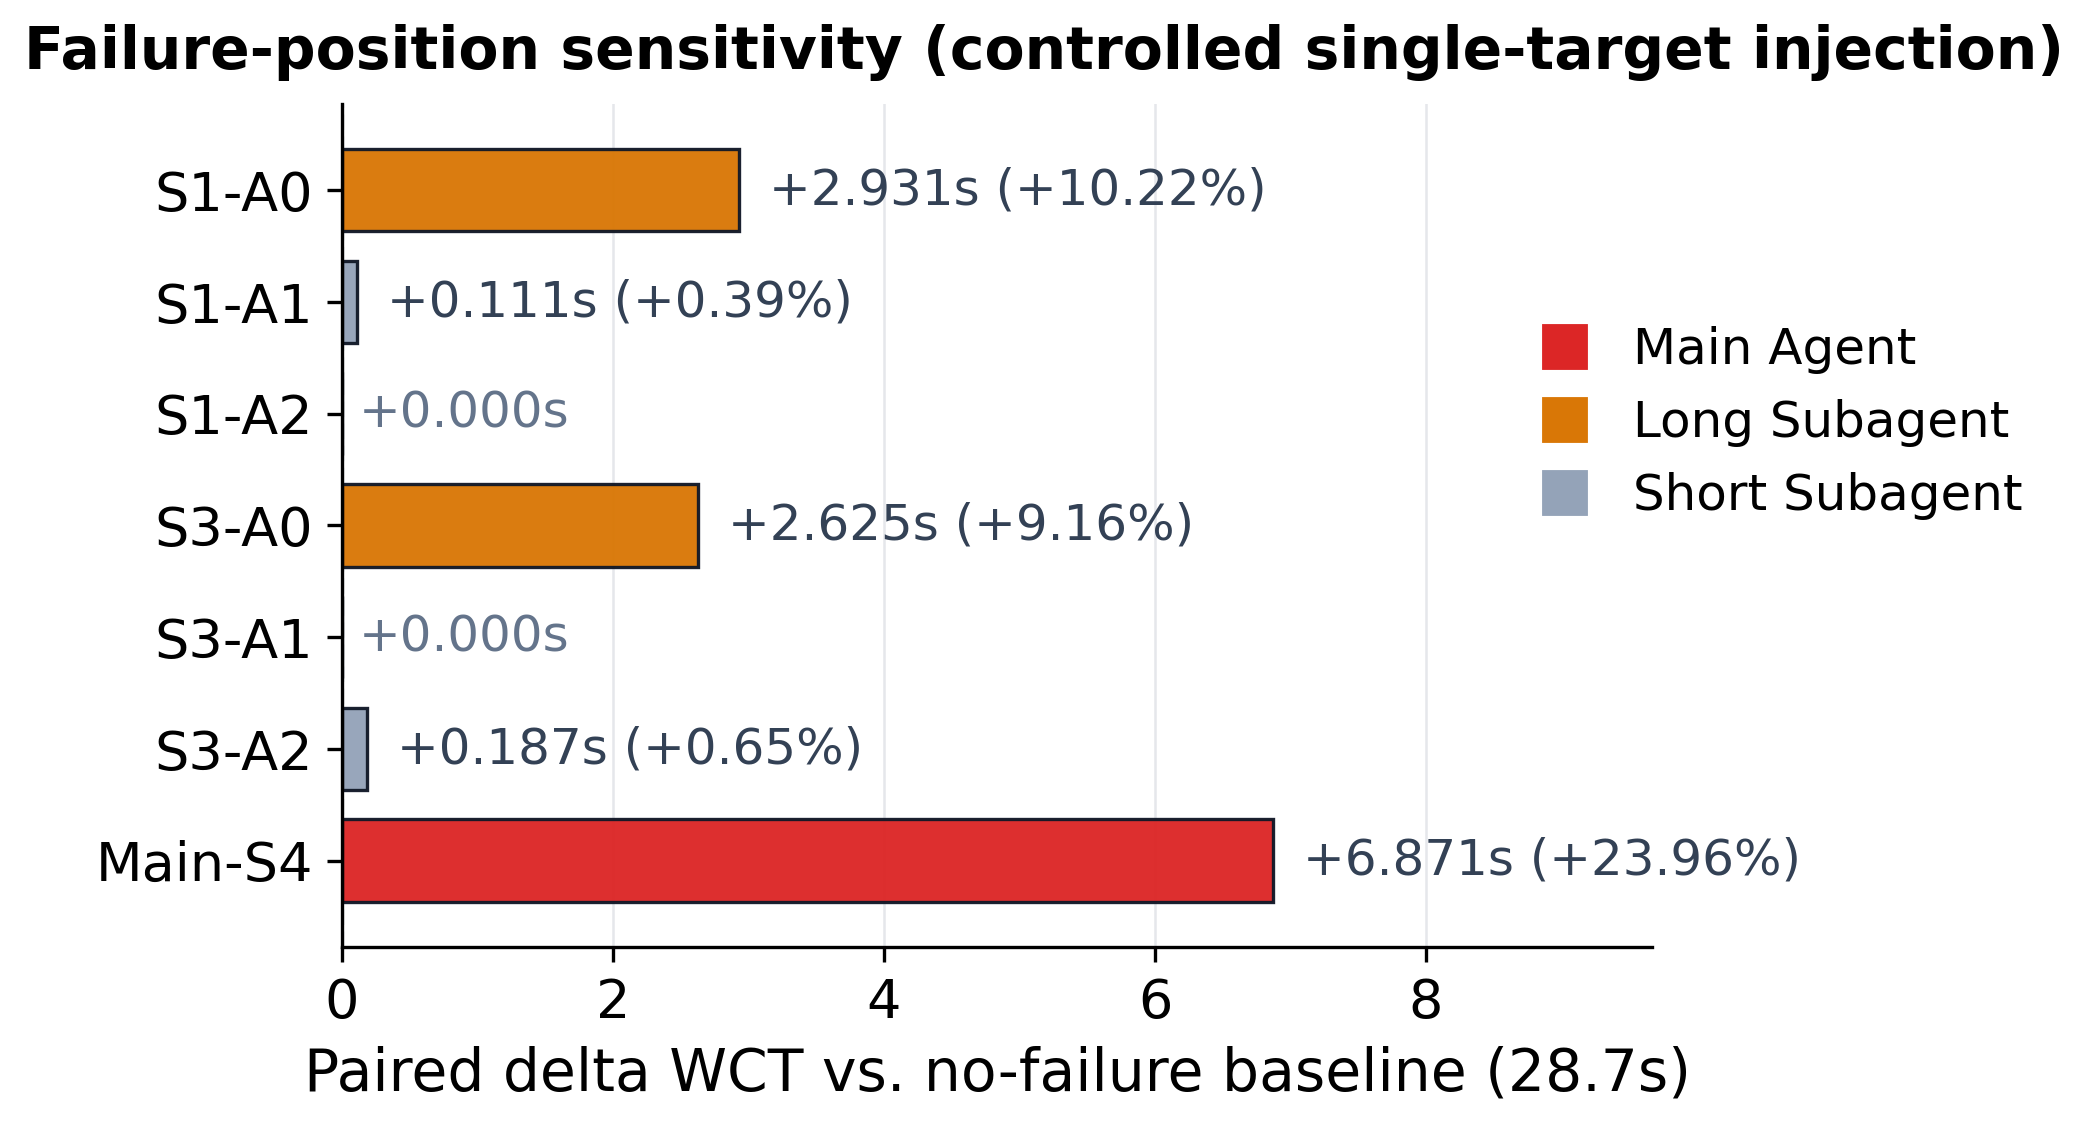
\includegraphics[width=0.88\textwidth]{../figures/motivation-failure-position.png}
  \caption{相同 KV 损失在不同工作流位置产生不同的 WCT 影响。}
  \label{fig:motivation-failure-position}
\end{figure}

\subsection{统一设计目标}

系统在满足正常路径开销约束的前提下，最小化 GPU failure 引起的工作流完成时间增量：
\begin{equation}
  \min\quad
  \mathbb E[\Delta \mathrm{WCT}_{\mathrm{failure}}]
  +\lambda_N C_{\mathrm{normal}},
  \label{eq:unified-objective}
\end{equation}
其中 $\Delta \mathrm{WCT}_{\mathrm{failure}}$ 是故障运行相对无故障运行的 WCT 增量，
$C_{\mathrm{normal}}$ 表示 KV 复制、空间预留和资源竞争对健康请求造成的开销。实际
控制中，Algorithm 2 以 chunk 的边际净收益近似该目标，Algorithm 3 在较慢时间尺度
调整可用容量。

\section{设计范围}

\begin{table}[H]
  \centering
  \caption{本阶段设计边界}
  \begin{tabularx}{\textwidth}{>{\bfseries}p{3.5cm}X}
    \toprule
    项目 & 设计基线 \\
    \midrule
    故障模型 & 底层 GPU fail-stop；故障 GPU 上的 KVCache 不可读取。 \\
    恢复方式 & 受影响请求整体重路由到健康 DP，不在不同 DP 间拼接执行中的 PP stage。 \\
    备份粒度 & KV chunk；请求生成过程中持续触发在线决策。 \\
    保护位置 & 其他 DP 的 GPU HBM、Host DRAM，或不增加副本并在故障时 Recompute。 \\
    并行拓扑 & 示例采用 DP=2、PP=2；同一 DP 的两个 PP scheduler/worker 独立运行。 \\
    资源控制 & 同一 DP 的全部 PP stage 共享一组 $\alpha_d$、$\beta_d$。 \\
    \bottomrule
  \end{tabularx}
\end{table}

\section{系统架构}

\begin{figure}[H]
  \centering
  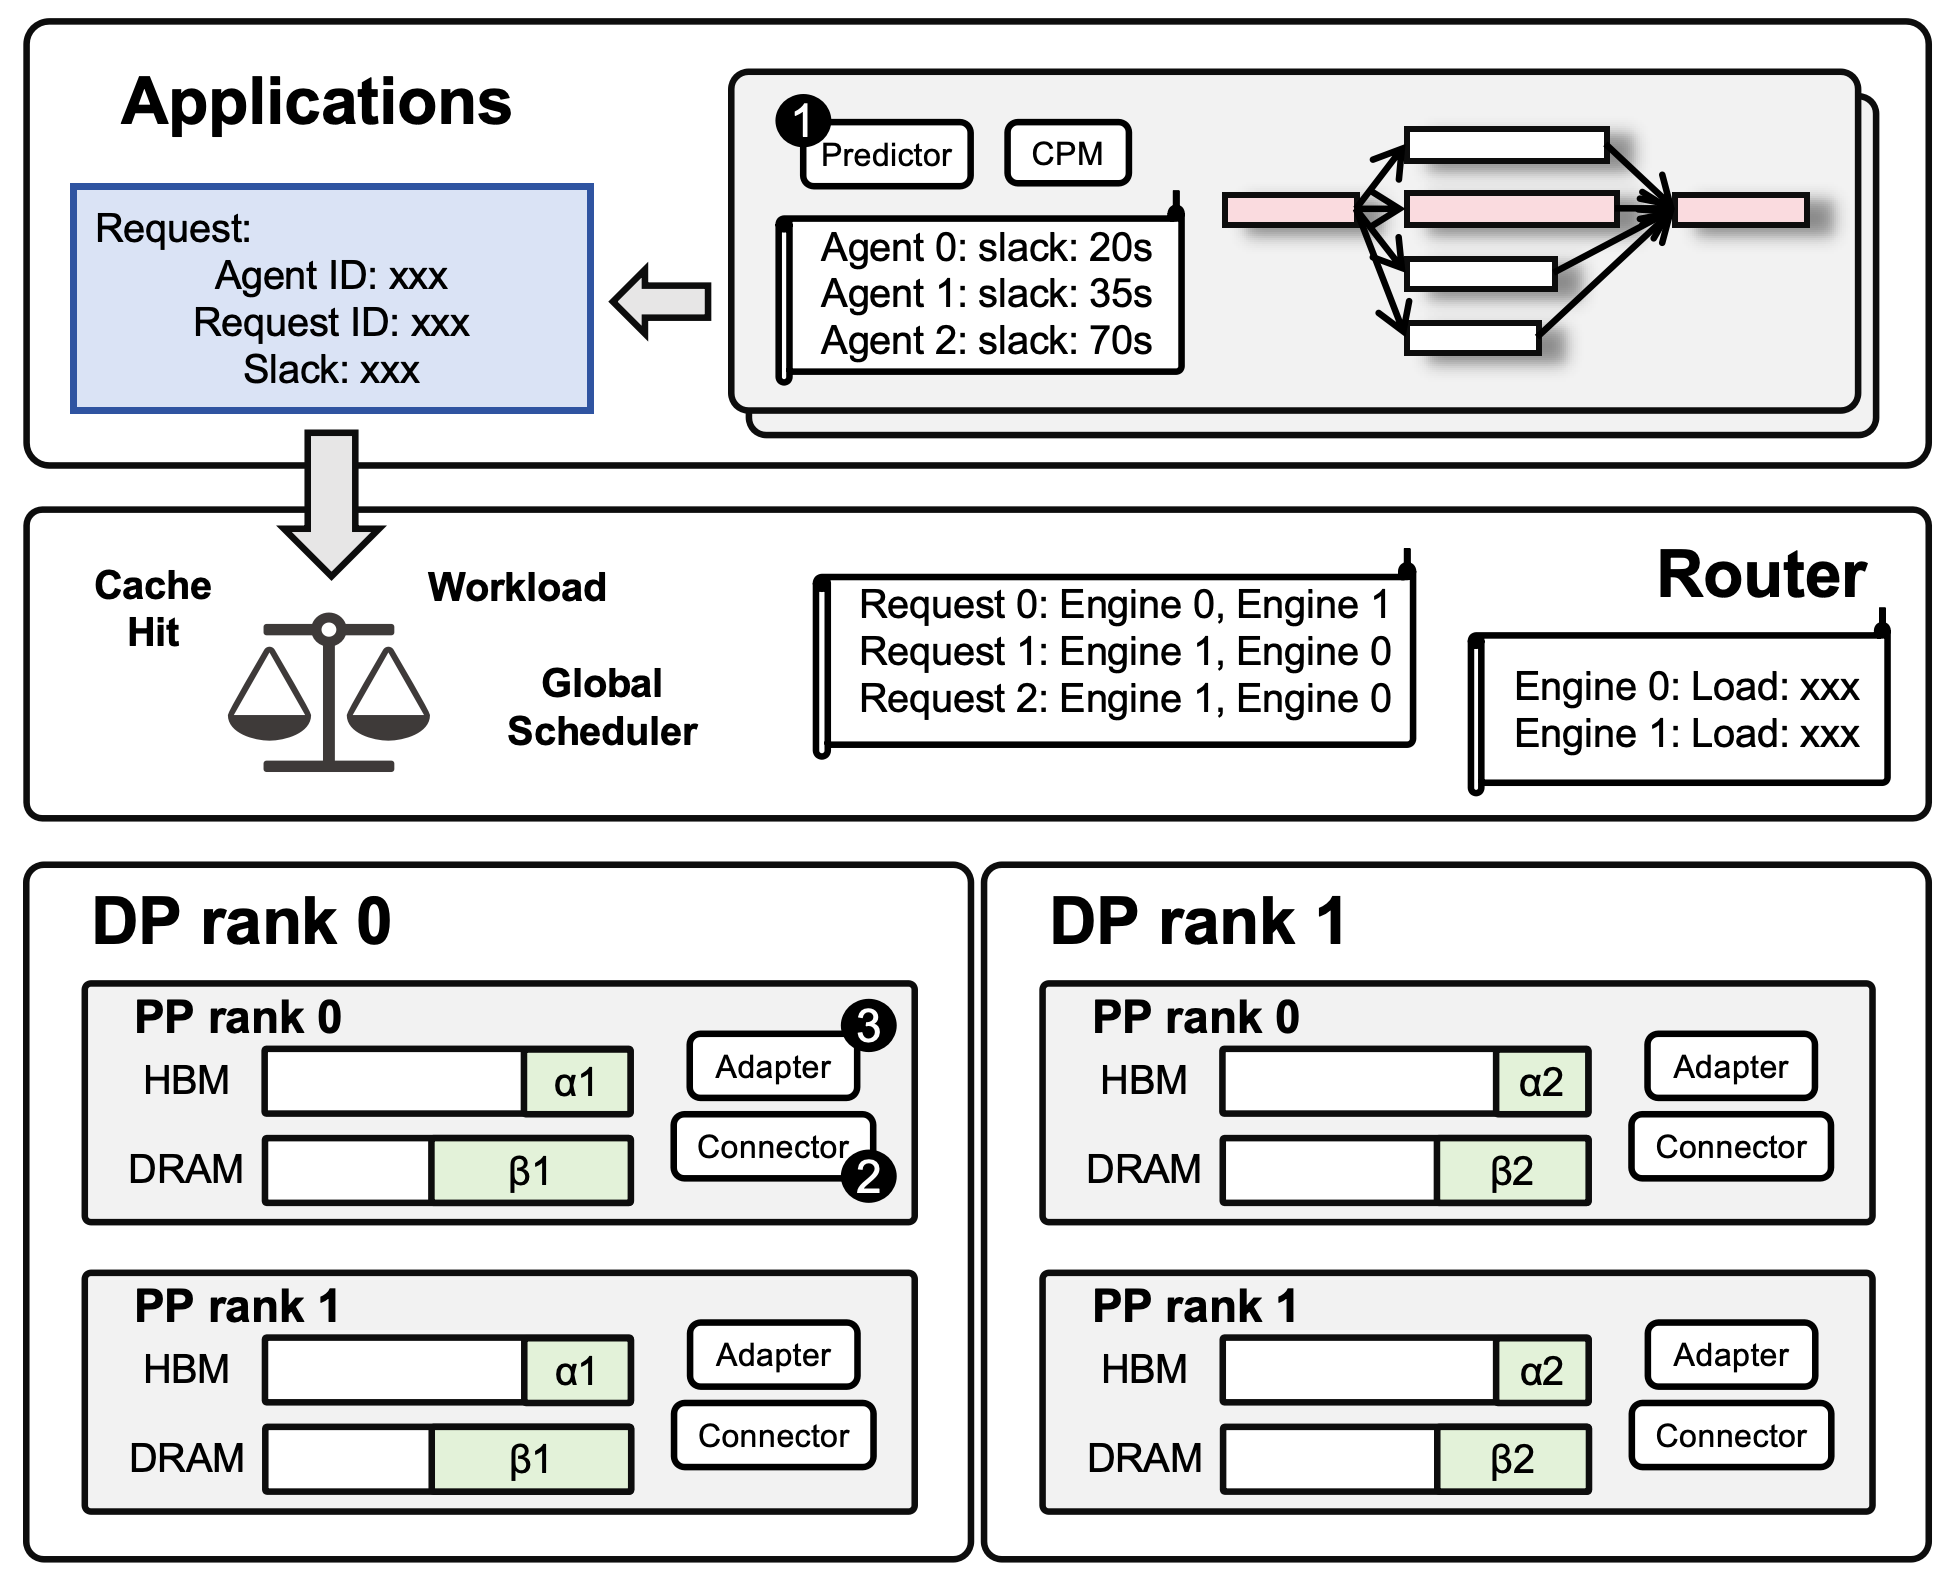
\includegraphics[width=0.76\textwidth]{../figures/aegiskv-ppt-system-architecture.png}
  \caption{ AegisKV 系统架构图。图中以 2 DP$\times$2 PP 为简化示意；
  实际部署可扩展到更大规模，此处保持每个 DP 统一管理 $\alpha/\beta$。}
  \label{fig:architecture}
\end{figure}

\begin{table}[H]
  \centering
  \caption{模块责任}
  \begin{tabularx}{\textwidth}{>{\bfseries}p{3.6cm}X}
    \toprule
    模块 & 责任 \\
    \midrule
    Workflow Handler & 维护已揭示工作流 DAG，预测节点时长，计算并下传请求 Slack。 \\
    Router & 选择执行 DP 和备份 DP；故障后把请求重路由到健康 DP。 \\
    AegisKV Controller & 执行 Algorithms 2/3，维护 chunk 放置状态和每 DP 资源预算。 \\
    Scheduler/worker & 每个 DP 内按 PP stage 独立执行推理并上报新增 KV chunk。 \\
    Connector & 执行同 PP stage 的跨 DP GPU 复制以及 GPU--Host 数据传输。 \\
    Host Pool & 提供受 $\beta$ 限制的 DRAM KV 备份空间。 \\
    \bottomrule
  \end{tabularx}
\end{table}

Controller 只传递元数据和决策，KV tensor 由 Connector 直接移动。Router 的执行路由
和备份路由是两个决策：前者关注正常推理负载和缓存命中，后者关注故障隔离、恢复
开销与目标 DP 的备份容量。

\section{Algorithm 1：工作流 Slack 计算}

\subsection{工作流执行图与时长预测}

在时刻 $t$，应用层把已经揭示的工作流表示为有向无环图
$G_t=(V_t,E_t)$。节点 $v$ 表示一次智能体调用，边表示调用依赖。对于每个尚未完成
的节点，GBDT 预测器根据当前可见特征 $\mathbf z_v(t)$ 估计剩余执行时间：
\begin{equation}
  \widehat d_v(t)=f_{\theta}(\mathbf z_v(t)).
  \label{eq:duration-predict}
\end{equation}
特征可包括节点类型、已完成轮数、prompt token、已生成 token、历史同类调用时长、
工具类型和当前服务负载。预测器只使用当时已经观察到的信息；未来工具结果和最终输出
长度不得作为输入。

\subsection{CPM 前向与反向计算}

对图中节点执行关键路径法（Critical Path Method, CPM）。前向遍历计算最早开始和
最早完成时间：
\begin{align}
  ES_v &= \max_{u\in\operatorname{pred}(v)} EF_u, \\
  EF_v &= ES_v+\widehat d_v .
  \label{eq:cpm-forward}
\end{align}
源节点的 $ES_v=0$。预测工作流剩余完成时间为
\begin{equation}
  \widehat T_W=\max_{v\in\operatorname{sink}(G_t)} EF_v .
\end{equation}
再从汇点反向遍历：
\begin{align}
  LF_v &= \min_{u\in\operatorname{succ}(v)} LS_u, \\
  LS_v &= LF_v-\widehat d_v ,
  \label{eq:cpm-backward}
\end{align}
其中汇点的 $LF_v=\widehat T_W$。节点的 Slack 为
\begin{equation}
  S_v=\max(LS_v-ES_v,0).
  \label{eq:node-slack}
\end{equation}
$S_v=0$ 表示节点位于当前预测关键路径；$S_v>0$ 表示该节点最多可额外延迟 $S_v$
而不改变当前预测 WCT。本文不再单独定义 critical score，Algorithm 2 直接使用 Slack
刻画故障延迟是否会暴露给工作流。

\subsection{请求级输出与更新时机}

一个节点可能包含多轮请求。对节点 $v$ 中当前请求 $r$，Handler 将剩余节点 Slack
映射为请求 Slack $S_r$，并在请求 metadata 中携带 workflow、agent、request 标识、
依赖状态和 $S_r$。以下事件触发重新计算：新节点或依赖边被揭示、tool call 返回、
节点完成、剩余时长预测明显变化。Algorithm 1 的输出是时间预算，不决定 KV 放置。

\section{Algorithm 2：基于边际恢复收益的分层备份}

\subsection{决策事件与候选动作}

请求 $r$ 的 KV 随 prefill/decode 持续增长。每当形成一个新 chunk $c$，Algorithm 2
对该 chunk 触发一次在线决策。候选动作集合为
\begin{equation}
  \mathcal A_{r,c}=\{\mathrm{GPU}(g),\ \mathrm{Host},\ \mathrm{Recompute}\},
  \label{eq:actions}
\end{equation}
其中 $g$ 是健康且与执行 DP 不同的候选备份 DP。$\mathrm{GPU}(g)$ 表示将 KV 写到
$g$ 的对应 PP stage HBM；Host 表示写到 DRAM 备份池；Recompute 表示不产生额外
副本，故障时重新计算。远端持久层可作为后续扩展，但不属于本阶段基线。

\subsection{恢复时间}

若当前请求已积累 $N_r$ 个需要恢复的前缀 token，完全重计算的时间写为
\begin{equation}
  T_{\mathrm{recompute}}(r)
  =t_{\mathrm{setup}}^{R}+N_r t_{\mathrm{token}}^{R}.
  \label{eq:recompute}
\end{equation}
$t_{\mathrm{setup}}^{R}$ 是重路由、重新准入和启动 prefill 的固定开销，
$t_{\mathrm{token}}^{R}$ 是每个前缀 token 的有效重算时间。

若从层级 $a\in\{G,H\}$ 恢复 $B$ 字节 KV，则
\begin{equation}
  T_{\mathrm{restore}}^{a}(B)
  =t_{\mathrm{setup}}^{a}
  +\frac{B}{\mathrm{BW}_{a}^{\mathrm{eff}}}
  +q_a .
  \label{eq:restore}
\end{equation}
$\mathrm{BW}_{a}^{\mathrm{eff}}$ 是包含并发争用后的有效带宽，$q_a$ 是目标 GPU 的
排队和重新准入开销。GPU backup 通常恢复最快；Host 需要 H2D，容量更大但恢复更慢。

\subsection{chunk 的边际恢复收益}

备份决策必须以 chunk 为粒度，而不是把请求级总收益平均分配给每个 chunk。设在决策
前请求的可复用 KV 为 $B_{r,c-1}$，将新 chunk 放到动作 $a$ 后可复用 KV 为
$B_{r,c}^{a}$。对应的故障恢复时间分别为 $T_{r,c-1}$ 和 $T_{r,c}^{a}$。Slack 能隐藏
的延迟不应计入 WCT 损失，因此定义
\begin{equation}
  L_r(T)=\max(T-S_r,0).
  \label{eq:visible-loss}
\end{equation}
若当前控制区间内执行 GPU 的故障概率为 $p_r^{\mathrm{fail}}$，新 chunk 放置到 $a$
的期望边际恢复收益为
\begin{equation}
  G_{r,c}^{a}
  =p_r^{\mathrm{fail}}
  \left[L_r(T_{r,c-1})-L_r(T_{r,c}^{a})\right].
  \label{eq:recovery-benefit}
\end{equation}
该式只计算“增加当前 chunk”带来的额外收益。随着请求增长，重算代价可能上升；但
越靠后的 chunk 剩余暴露时间通常更短、累计占用更高，因此其边际价值不必然增加。

\subsection{备份成本与净价值}

动作 $a$ 的备份成本由三部分组成：
\begin{equation}
  C_{r,c}^{a}
  =C_{\mathrm{copy}}^{a}
  +C_{\mathrm{capacity}}^{a}
  +C_{\mathrm{interference}}^{a}.
  \label{eq:backup-cost}
\end{equation}
$C_{\mathrm{copy}}^{a}$ 由 chunk 字节数、P2P/D2H 有效带宽和传输排队决定；
$C_{\mathrm{capacity}}^{a}$ 表示 KV 在 HBM 或 DRAM 中驻留的机会成本；
$C_{\mathrm{interference}}^{a}$ 表示复制对正常 prefill/decode、copy engine 和链路的
可见干扰。已经驻留的 chunk 不重复收取复制成本，但仍持续占用容量。

净价值和单位容量价值密度为
\begin{equation}
  V_{r,c}^{a}=G_{r,c}^{a}-C_{r,c}^{a},
  \qquad
  \rho_{r,c}^{a}=\frac{V_{r,c}^{a}}{B_{r,c}}.
  \label{eq:value-density}
\end{equation}
Algorithm 2 首先排除故障域不独立、目标 DP 无恢复能力、容量不足或带宽门禁不满足的
候选，再选择 $\rho$ 最大的动作。若最优 $V\le 0$，输出 Recompute；若容量足够且
$V>0$，接纳该 chunk；若容量不足，则仅当新 chunk 的 $\rho$ 高于当前最低价值条目时
执行替换，否则不备份。该流程是答辩方案中的在线 value-density 策略，不声称对未知
未来请求和故障序列达到全局最优。

\subsection{对 Algorithm 3 的反馈}

Algorithm 2 在每个控制窗口分别为 GPU 和 Host 统计：
\begin{itemize}
  \item $D$（Demand）：净价值为正、希望接纳的 chunk 数、字节数和价值；
  \item $U$（Usage）：实际接纳并持续占用的 chunk 数、字节数和实现价值；
  \item $O$（Overflow）：因容量或正常路径门禁未能接纳的字节数及损失价值。
\end{itemize}
同时记录复制带宽、正常请求 slowdown、恢复命中和重算 token。$D/U/O$ 不能只计请求
数，因为不同 chunk 大小和保护价值差异很大。

\section{Algorithm 3：HBM/DRAM 备份容量控制}

\subsection{每 DP 统一的双层预算}

对 DP $d$，定义
\begin{equation}
  M_{d}^{G}(K)=\alpha_d^K M_{d,\max}^{G},
  \qquad
  M_{d}^{H}(K)=\beta_d^K M_{d,\max}^{H},
  \label{eq:alpha-beta}
\end{equation}
其中 $M_{d}^{G}$ 是 GPU HBM 备份预算，$M_{d}^{H}$ 是 Host DRAM 逻辑预算。
$\alpha_d,\beta_d\in[0,1]$。同一 DP 的所有 PP stage 使用相同的 $\alpha_d$ 和
$\beta_d$；每个 stage 仍需按自身物理余量执行硬约束。若多个 DP 共享同一 Host
内存池，底层分配器还需保证各 DP 的 $\beta$ 配额之和不超过节点物理容量。

\subsection{时间窗口与状态}

Algorithm 2 在窗口 $K$ 内随 chunk 到达实时决策，Algorithm 3 只在窗口边界更新一次
预算。窗口可按固定时长 $T_K$ 定义，也可在达到最小持续时间后由 chunk 事件数触发；
原则是既要积累足够反馈，又不能让负载变化长期得不到响应。窗口状态为
\begin{equation}
  X_d^K=(D_d^K,U_d^K,O_d^K,
  P_{\mathrm{infer},d}^K,P_{\mathrm{copy},d}^K,
  \alpha_d^K,\beta_d^K),
  \label{eq:window-state}
\end{equation}
其中 $P_{\mathrm{infer}}$ 表示正常推理压力，$P_{\mathrm{copy}}$ 表示复制和链路压力。

\subsection{候选动作与更新目标}

答辩方案采用离散增量控制：
\begin{equation}
  \Delta\alpha_d,\Delta\beta_d
  \in\{-0.10,-0.05,0,+0.05,+0.10\}.
  \label{eq:budget-actions}
\end{equation}
对每个可行候选，控制器预测下一窗口未满足保护价值、正常路径开销、空置预算和调整
成本，并选择
\begin{equation}
  (\alpha_d^{K+1},\beta_d^{K+1})
  =\arg\min_{(\alpha,\beta)\in\mathcal B_d^K}
  \left[
    \lambda_O\widehat O_d(\alpha,\beta)
    +\lambda_N\widehat C_{\mathrm{normal},d}(\alpha,\beta)
    +\lambda_I\widehat C_{\mathrm{idle},d}(\alpha,\beta)
    +\lambda_S C_{\mathrm{switch}}
  \right].
  \label{eq:alg3-objective}
\end{equation}
$\mathcal B_d^K$ 由 HBM/DRAM 物理上限和正常推理安全余量确定。$\widehat O$ 衡量预算
不足会丢失多少正净收益；$C_{\mathrm{normal}}$ 衡量挤压正常推理和复制干扰；
$C_{\mathrm{idle}}$ 防止长期保留大量未使用空间；$C_{\mathrm{switch}}$ 抑制频繁抖动。

直观上，$O$ 高、正常负载低时提高相应预算；$D$ 和 $U$ 长期较低时降低预算；若
$O$ 高但正常推理或复制链路已过载，则不盲目扩容，而应让 Algorithm 2 更多选择 Host
或 Recompute。窗口 $K$ 的观测只决定 $K+1$，避免用同一批反馈同时产生和评价动作。

\section{三个算法的闭环与运行流程}

\subsection{正常路径}

\begin{enumerate}
  \item Workflow Handler 更新已揭示 DAG，Algorithm 1 计算请求 Slack 并随请求下传。
  \item Router 选择执行 DP，并为需要 GPU 保护的请求确定候选备份 DP。
  \item 新 KV chunk 到达时，Algorithm 2 比较 GPU、Host 与 Recompute 的边际净价值。
  \item Connector 按决策执行同 PP stage P2P 或 D2H；Controller 更新放置状态和 $D/U/O$。
  \item 窗口结束后，Algorithm 3 更新各 DP 的 $\alpha/\beta$，供下一窗口使用。
\end{enumerate}

\subsection{GPU failure 恢复}

执行 GPU 失效后，Router 停止向故障 DP 发送请求，并把受影响请求整体重路由到健康
DP。恢复总时延为
\begin{equation}
  T_{\mathrm{retry}}
  =T_{\mathrm{detect}}+T_{\mathrm{route}}
  +T_{\mathrm{restore}}+T_{\mathrm{recompute\ suffix}}
  +T_{\mathrm{queue}}.
  \label{eq:retry}
\end{equation}
目标 DP 优先复用其 HBM 中的备份 KV；否则从 Host DRAM 执行 H2D；未覆盖部分重新
prefill。系统记录恢复来源、复用 token、重算 token、retry 时延和最终 WCT 增量。

\section{接口与可观测性}

\begin{table}[H]
  \centering
  \caption{关键接口和字段}
  \begin{tabularx}{\textwidth}{>{\bfseries\raggedright\arraybackslash}p{4.2cm}X}
    \toprule
    接口/事件 & 关键字段 \\
    \midrule
    RegisterRequest & workflow/agent/request id、DAG 节点、Slack、执行 DP。 \\
    ChunkReady & request/chunk id、PP stage、token range、KV bytes。 \\
    PlacementDecision & backup DP、GPU/Host/Recompute、预期收益、成本、$\rho$。 \\
    PlacementComplete & 实际位置、完成时间、占用字节和传输开销。 \\
    BudgetUpdate & DP id、$\alpha$、$\beta$、窗口编号、调整原因。 \\
    Failure/Retry & 故障 GPU、重路由 DP、恢复来源、复用/重算 token、WCT 增量。 \\
    \bottomrule
  \end{tabularx}
\end{table}

\section{初步结果与验收要求}

现有 SGLSim 初步回放对比 AegisKV 与 No Backup 的 WCT CDF，并统计 retry 请求的 KV
复用。该结果用于确认指标链和实验流程可运行，不等同于完整算法已经取得最终收益。

\begin{figure}[H]
  \centering
  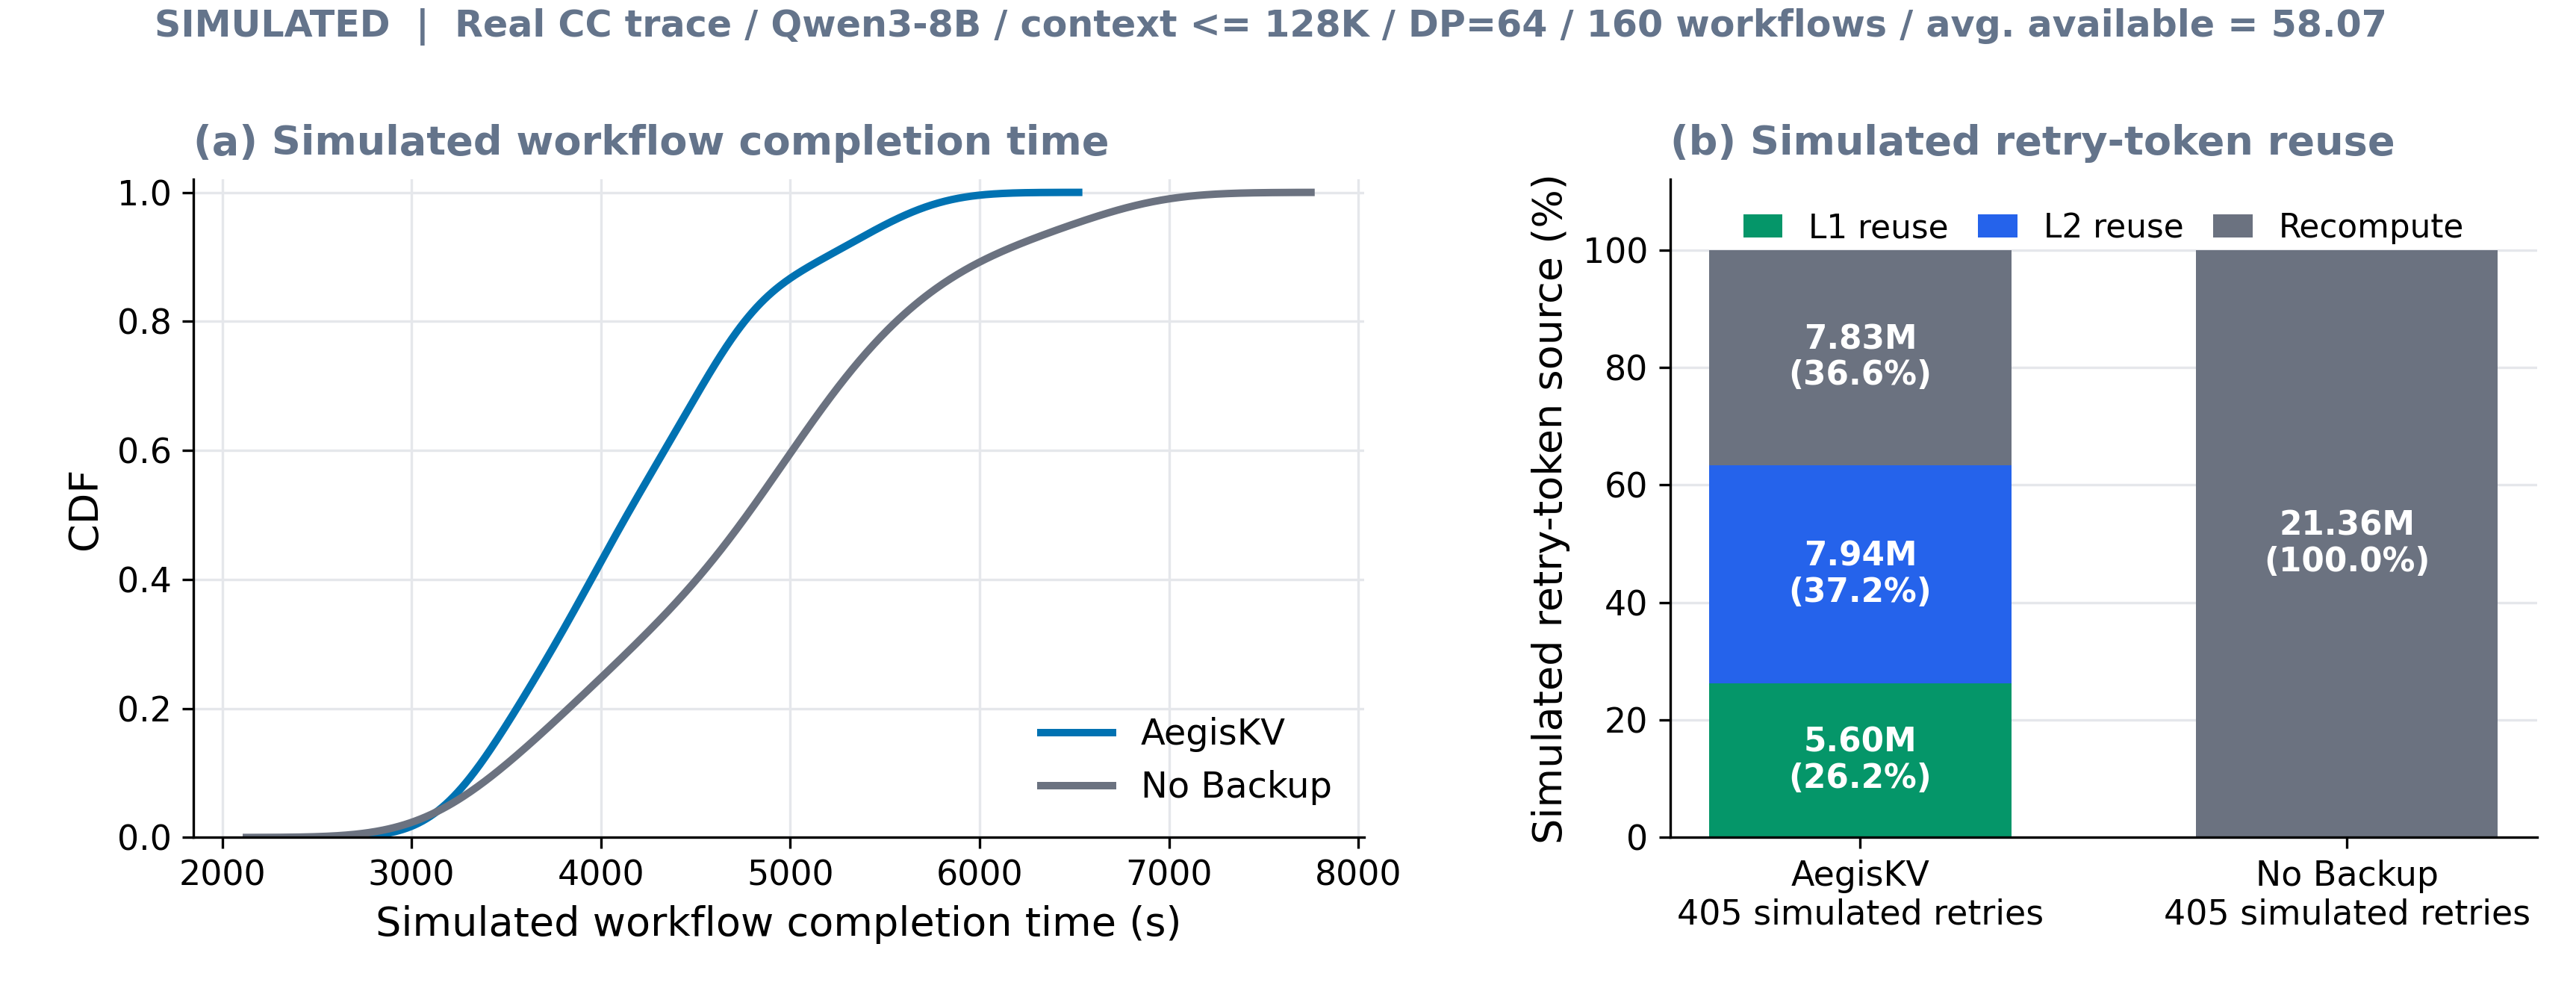
\includegraphics[width=0.96\textwidth]{../figures/preliminary-wct-kv-reuse.png}
  \caption{初步 SGLSim WCT CDF 与 retry KV reuse 结果。}
  \label{fig:preliminary-result}
\end{figure}

\begin{figure}[H]
  \centering
  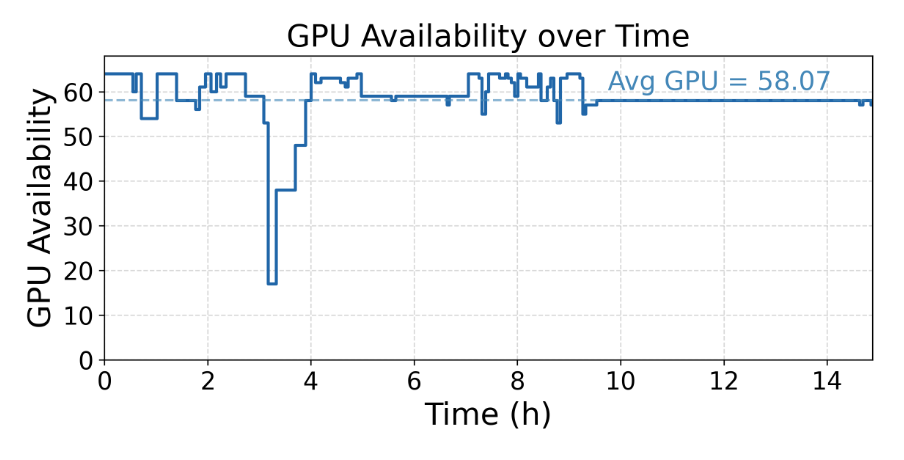
\includegraphics[width=0.68\textwidth]{../figures/motivation-gpu-availability.png}
  \caption{初步模拟使用的 GPU availability 轨迹。}
  \label{fig:preliminary-availability}
\end{figure}

\begin{longtable}{p{2.1cm}p{6.0cm}p{6.3cm}}
  \caption{核心验收项}\label{tab:acceptance}\\
  \toprule
  编号 & 检查内容 & 通过条件 \\
  \midrule
  \endfirsthead
  \toprule
  编号 & 检查内容 & 通过条件 \\
  \midrule
  \endhead
  AC-01 & DP$\times$PP 拓扑 & DP=4 时每个 DP 启动四个独立 PP scheduler/worker，身份和生命周期可核对。 \\
  AC-02 & 工作流元数据 & workflow/agent/request id 与 Slack 可从应用层传到 Router 和推理层。 \\
  AC-03 & chunk 级决策 & 每个新增 chunk 记录 GPU/Host/Recompute 候选、收益、成本和最终动作。 \\
  AC-04 & 同 stage 传输 & GPU backup 仅在相同 PP stage 间复制，实际目标 DP 与记录一致。 \\
  AC-05 & 双层预算 & 每 DP 一组 $\alpha/\beta$；窗口 $K$ 的 $D/U/O$ 可追溯到 $K+1$ 的调整。 \\
  AC-06 & GPU failure 恢复 & 整请求重路由，GPU/Host 复用与 suffix 重算 token 均可核对。 \\
  AC-07 & 正常路径开销 & 报告无故障吞吐、WCT、P99 与复制带宽，且不超过预先设定门限。 \\
  AC-08 & 正式实验 & 每个主要配置不少于 100 个 workflow，采用 paired No Backup 并给出置信区间。 \\
  \bottomrule
\end{longtable}

正式结果包应包含冻结的 workload/config、代码和模型哈希、请求级事件、failure/retry/
restore 记录、$D/U/O$ 窗口统计、聚合脚本、图表输入数据和复现实验命令。

\section{风险与后续工作}

\begin{itemize}
  \item \textbf{时长与故障概率误差：}通过时间预测校准、参数敏感性和 oracle 对照评估。
  \item \textbf{正常路径干扰：}使用真实 P2P/D2H/H2D 测量标定复制和恢复模型，并设置硬门禁。
  \item \textbf{在线 value-density 局限：}与无保护、全量 Host、固定 $\alpha/\beta$ 和离线 oracle 做消融。
  \item \textbf{控制稳定性：}评估窗口大小、调整步长和切换惩罚，避免预算频繁振荡。
  \item \textbf{范围扩展：}远端存储、多故障和节点级故障留作后续工作，不混入当前基线。
\end{itemize}

\section{结论}

\systemname{} 通过 Algorithm 1 的工作流 Slack、Algorithm 2 的 chunk 级 GPU/Host/
Recompute 选择，以及 Algorithm 3 的 per-DP $\alpha/\beta$ 闭环控制，在正常服务
开销和 GPU 故障恢复收益之间进行权衡。本文给出了与答辩方案一致的系统边界、公式、
数据流和验收条件；性能结论仍需由完整实现和正式 paired 实验验证。

\clearpage
\bibliographystyle{unsrt}
\bibliography{references}

\end{document}
